%aum ghanaathipathaye namaha
%sri rama jeyam

\section{Structural Modeling} \label{subsec:abs_sem_mod}
%The key problem of state-based semantic modeling is that it is too low-level, which may lead to the same semantics model from totally different binary codes.

%Therefore, matching using state-based semantic information will give too many false positives, especially when the program segment is small.
%\ly{the following paragraph can be removed.}
%Due to the challenges of state-based semantic modeling mentioned in Section \ref{sec:prob_state}, many false positives might be produced during the matching process.
%In addition, with the presence of an uninterpreted system API, the state-based semantic models are incapable of capturing the precise semantics.
%In fact, it is impossible to model the machine state transitions involving system API using static analysis unless function  summaries are available for all system APIs across different OSs.

To complement state-based semantic modeling, we introduce an idiom based modeling to capture structure and the high level behaviour of the binary.
To this end, we leverage the following analysis --- \idiomDep{(1)} idiom analysis that looks for familiar and recurring machine code patterns that are already observed in the majority of binaries from real world. \idiomDep{; and (2) idiom dependency analysis captures the dependency relationship between the extracted idioms.}

%In addition, even if the program segment is free of any uninterpreted system API, if it is too small, i.e., too few instructions, the state-based models will become unreliable, where two totally irrelevant code segments might result in an identical post-state (i.e., machine state after execution) given the same pre-state (i.e, machine state before execution)

%\begin{figure}[!h]
%\scriptsize
%  \begin{subfigure}[b]{0.5\linewidth}
%    \centering
%   % \includegraphics[width=0.75\linewidth]{srj-figures/srj-hierarchy-2.png}
%    \raggedright{\textbf{\texttt{
%    \\
%    	add  ebx, eax\\
%    	add  ebx, 2h\\
%   		shl  ebx, 2\\
%   		test ebx, 4\\
%   		jz ecx\\
%    }}}
%    \caption{\small{}}
%   \label{fig:traceleta}
%    \vspace{1ex}
%  \end{subfigure}%%
%  \begin{subfigure}[b]{0.5\linewidth}
%    \centering
%      \raggedright{\textbf{\texttt{
%    \\
%    	mov eax, [0x1234]\\
%    	lea	ebx, [eax+0x4]\\
%   		mov	eax, [ebx]\\
%   		cmp eax, 0\\
%   		jz edx\\
%    }}}
%    \caption{\small{}}
%    \label{fig:traceletb}
%    \vspace{1ex}
%  \end{subfigure}
%  \caption{Code segments that result in identical post-state given the same pre-state even though their high-level intentions are not comparable\\}
%  \label{fig:ex-tracelet}
%\end{figure}
%
%For example, given the same pre-state, the code segments given in figure~\ref{fig:abs} will result in an identical post-state even though their high-level intentions are not comparable. That is, assuming all the registers, flags and memory locations are assigned the value `0' in the pre-state. After execution, the post-state for code segment (a) will be: \texttt{ebx} register will hold the value `4', while all other registers, flags and memory locations will retain their pre-state values. Similarly, in the post-state for code segment (b), the \texttt{ebx} register will hold the value `4' and all the other registers, flags and memory locations will retain their pre-state values.

%This behaviour is undesirable especially, when searching for potential vulnerable code segments in the target binary, where this will lead to high false positive rate. Hence, in \tool, we complement state-based models with abstract semantic models, where state-based models capture the low-level semantics of the code segment and using abstract semantic models we try to capture the high-level objective (or behaviour) of the code segment. The features extracted from these two models are complement to each other.
%To this end, we leverage on two types of analysis to infer the high-level computations of the code segments: (1) machine code \textit{idiom analysis}, and (2) \textit{dependency analysis}. Idiom analysis try to look for familiar and recurring machine code patterns that are already observed in the majority of the binaries in the wild, whereas, dependency analysis captures the relationship (i.e., dependency) between the extracted idioms.

%As discussed in section~\ref{sec:prob_state}, program segments (or functions) perform a series of computations through which they accomplish their objectives (e.g., create a buffer in the memory, send data over network). To understand the high-level objective (or behaviour) of a program segment, it is essential to capture the computations underneath it.

\subsection{Idioms} \label{subsec:idiom_ana}
Motivated by source code idioms~\cite{allamanis2014mining}, we find that the same concept applies in binaries, i.e., the recurring patterns of binary instructions reveal some fixed semantics.
%The presence of idioms, in the program segment, helps to understand the machine code better.
For example, the idiom given below indicates that the code segment under analysis sets up the stack frame in the function prologue.
\begin{itemize}
\centering
\itemsep-0.5em
  \item[] $\mathtt{push \;\;ebp; \quad mov \;\; ebp, esp;}$
 % \item[] $\mathtt{mov \quad ebp, esp}$
\end{itemize}

In addition to revealing high-level meaning, idioms can also explain the compilation process.
The presence of code segment (in Fig.~\ref{fig:gcc_ssp}) in the function prologue and epilogue ensure that the stack integrity is not violated, where it is automatically included by the compiler (in this case, $\mathtt{gcc}$) when stack smash protection compiler feature is enabled (using either -$\mathtt{fstack}$-$\mathtt{protector}$-$\mathtt{all}$ or -$\mathtt{fstack}$-$\mathtt{protector}$ flag). Generalizing the code segments, shown in Fig.~\ref{fig:gcc_ssp}, into an idiom helps an analyst to identify that binaries are protected by the stack smash protection (SSP) compiler feature. %\footnote{Stack smash protection is a first line of defence that only detects the stack buffer over runs and does not prevent them. This protection can be beaten by correctly identifying the stack canary~\cite{pincus2004beyond}.}. %Hence, idioms can also be used to pre-filter the candidate target functions that are of analyst's interest.
%help in pre-filtering the target candidates, especially in vulnerability signature matching. For example, consider the following program segment:
\begin{figure}[t]
\small
\begin{itemize}
%\centering
\itemsep-0.2em
  \item[] $\mathtt{mov  \quad eax, gs:20 \quad}$
  \item[] $\mathtt{mov \quad [ebp-12], eax}$
  \makebox(0,0){\put(0,2.2\normalbaselineskip){%
               $\left.\rule{0pt}{1.1\normalbaselineskip}\right\}$ function prologue}}
  \item[] $\mathtt{\ldots \quad\quad\quad}$
  \item[] $\mathtt{\ldots\quad\quad\quad}$
  \item[] $\mathtt{mov  \quad eax, [ebp-12]}$
  \item[] $\mathtt{xor \quad eax, gs:20 \quad\quad}$
  \makebox(0,0){\put(0,2.2\normalbaselineskip){%
               $\left.\rule{0pt}{1.1\normalbaselineskip}\right\}$ function epilogue}}
\end{itemize}
  \caption{Code generated by \texttt{gcc} to enable SSP compiler feature}% (using either -$\mathtt{fstack}$-$\mathtt{protector}$-$\mathtt{all}$ or -$\mathtt{fstack}$-$\mathtt{protector}$ flag).}
  \label{fig:gcc_ssp}
\end{figure}
%in addition to understand the high-level behaviour,

Hence, using idioms, we can capture various interesting concepts and properties in a program segment, which in return, help us to understand the high-level behavior. %We formally define idiom as follows:
%\ly{machine code below is same as the instructions in sec 4? or QFBV? make sure the consistancy} \note{This is pure machine code. QFBV is redundant. I'll remove QFBV in sec 4}
%\begin{mydef}
%\emph{(\textbf{Idiom})} A recurring machine code pattern that has a single semantic purpose, which may be unified across different architectures and OSs.
%\end{mydef}
Let $\mathcal{I}$  be a partial trace, consisting of a sequence of \emph{normalized} instructions $\langle i_1,i_2, ..., i_n \rangle$, and $n$ be an $n$-gram model ($n$-length sub-sequence in $\mathcal{I}$, e.g., 3-gram model of $\langle{i_2,i_3,i_4} \rangle$) . We also define $\mathcal{N}$ =  $\{n_1,n_2, ..., n_m \}$ as the set of all possible $n$-gram models on $\mathcal{I}$ such that $\mathcal{N} \subseteq \powerset{\mathcal{I}}$.
Normalized instructions refer to assembly instructions abstracted away from volatile/noisy artifacts such as immediate values and absolute memory locations (see Section~\ref{subsubsec:func_norm} for details).

% \vspace{-2mm}
 \begin{mydef}
\emph{(\textbf{Idiom})} A $n$-gram model $n_i$  is considered as an idiom \textbf{iff} $n_i$ surpasses the minimum threshold of recurring probability $t$, which is predefined according to the observation in real-word binaries, and holds a valid high-level meanings.
\end{mydef}
% \vspace{-2mm}

 According to the above definition, we look for idioms observed in real-world binaries and map them to a valid unified high-level meaning (i.e., the tasks achieved by the idiom). % ---  machine code patterns or frequent instruction sequences --- that are frequently
 Note that the instruction sequences (i.e., idioms) are architecture and OS dependent. However, their high-level meanings are usually agnostic to differences in architectures and OSs.

 For example, an instruction sequence that implements the system API invocation in one architecture is totally different from that in another architecture, depending on the calling conventions used (discussed in Section~\ref{subsubsec:archi_plat_dep}). However, at high-level they all achieve the same objective by invoking the same or similar system APIs.
%\note{Similarly, the system APIs too unified based on the objectives accomplished}
%\note{Similarly, the system APIs, that are used to accomplish similar objectives, can vary from OS (or platform) to OS and between different versions of the same OS, hence they too need to be abstracted}.
Therefore extracting idioms, from various architectures and OSes, with mapping to a unified high-level meaning, helps to summarize the behavioral semantics of the program segment (or function) under analysis.

%\ly{Note that some idioms may be environment specific, e.g., . We argue that these idioms are also useful, e.g., to filter the relevant idioms to fast matching.}
Note that some machine code patterns appear only in certain type of architecture (or OS) and hence, cannot be unified across architectures and OSs. However, we still consider them as idioms as they can be used in the analysis where only the relevant architectures (or OSs) are involved. For example, stack split (or segmentation) capability is available only in \texttt{gcc} compiler (using \texttt{-fsplit-stack} flag) and for x86 32bit binaries only, and hence the machine code pattern that implements the stack split functionality cannot be unified across architecture (or OS). However, it can be useful for analysis that involve x86 32bit binaries compiled for Linux.

%\xyx{To sum up, idioms, as recurring binary code patterns, are not cross architecture or platform on their own. The high-level concept cross architecture and platform is attained by unifying similar idioms in a manual vetting process. For idioms that are architecture- or platform- specific, their high-level concepts are also identified for different types of analysis. Hence, we list the categories of idioms and their possible applications.}

%It is important to note that recurring machine code patterns are extracted per architecture and platform basis, and through a manual vetting process (discussed in section~\ref{subsec:idi_extr}) we try to understand the high-level meaning of the code pattern and unify across architecture and platform.


%An idiom is a syntactic fragment that recurs  frequent across binaries and has a single semantic purpose \cite{allamanis2014mining}.
\subsubsection{Idiom Classification} \label{sec:idiom:def}
The structural model of a binary program can be characterised by various properties such as data structures used (e.g., array, structure, etc.),
%data type information (e.g., \texttt{int}, \texttt{float}, $\ldots$),
variable types involved (e.g., local and global variables), %system APIs invoked during the computation (e.g., \texttt{strlen}, \texttt{memcpy}, etc.),
and other structural properties. In addition, sometimes, compilers influence a computation through the various compiler features. % such as stack smash protection (using \texttt{-fstack-protector} flag in \texttt{gcc}).

%\ly{need to give one example for each type} \note{will update in table 2}
To reflect different aspects of the structural information,
we classify idioms into three major types based on the nature of information related. These idioms together can be considered as the concrete implementation of function $f^{p}_{a}(\mathcal{I})$ defined in Definition~\ref{def:comp_sim}.
Note that this classification is not the only way or complete way to model different concepts in behavior models.
The different applications of the binary searching may require different idioms to be used.
Further more, the idioms can be extended based on demands.

%\st{(1) semantic idioms, (2) structural idioms, and (3) compiler idioms, where each idiom type captures different computation properties. Semantic idioms capture the system API related information that is ignored in the state-based semantic models (discussed in section . Similarly, structural idioms capture the computation properties such as data structures, variable types and other structural aspects like function boundary details and register access patterns. Finally, compiler idioms capture the compiler features --- code portions that are included by the compiler during compilation process}.

%\note{\textbf{examples will update in table 2 for each type of idiom}}
%
%\begin{itemize}
%
%\item \textbf{Semantic idiom}: This type of idioms provide the semantic details of the code segment under analysis, where it captures the system API invocation patterns. System API, in general, indicates the type of operation carried out by the program. For example, presence of \texttt{strlen} system API indicates that the program handles strings, more specifically, string arithmetic. In addition, co-occurrence of two or more system API gives more insight into the high-level intentions of the program segment. For instance, presence of \texttt{strlen} and \texttt{memcpy} system APIs in a code segment indicates buffer manipulation operation involving string arithmetic. Hence, learning the system API invocation patterns from existing binaries and generalizing them in to meaningful semantic idioms will help analysts to understand the high-level intentions of binary programs under evaluation.  It is important to note that to accommodate cross-platform analysis, we apply two levels of abstraction for system APIs (discussed in detail later in the section).
%
%\item \textbf{Structural idiom}: These idioms helps to identify the structural details and code properties of the program segment. For example, presence of an instruction pattern \texttt{sub esp,Imm} in a code segment compiled for \texttt{x86 32-bit} architecture indicates stack frame size manipulation operation. In addition, also capture other common structural properties such as save/restoring of callee/caller-save registers\footnote{Callee-saved registers are used to hold long-lived values that should be preserved across calls. Similarly, caller-saved registers are used to hold temporary quantities that need not be preserved across calls.}, presence of function prologue/epilogue and presence of loops. Further structural idioms also try to capture the code properties such as local/global variable access, function parameter manipulation and array manipulation.  It is important to note that structural idioms are architecture dependent, however, their high-level meanings are unified across architectures. Further, one cannot precisely extract code properties using structural idioms, for example, using only light-weight static analysis, it is impossible to distinguish between a string and an array\footnote{\note{mention how they are represented in memory}}. However, in our analysis, if there is a consecutive memory access pattern, we try to guess the data structure based on the co-occurrence of other idioms, that is, we map consecutive memory access pattern to a string given the presence of string related system APIs in the code segment. This approach is not precise but works relatively well and very scalable compare to more heavy-weight program analysis techniques~\cite{balakrishnan2007divine}.
%
%\item \textbf{Compiler idiom}: These idioms helps to identify the additional code included by the compiler during compilation process. For example, there are more than \note{XX} compiler options available for \texttt{gcc} that a programmer can choose from when compiling her code, where most of the features insert additional code into the compiled binary. One such example is the stack smash protection (SSP) code included in the function prologue and epilogue. Interestingly, some compiler idioms helps to understand more about the program, for example, presence of SSP in selected functions (i.e., -$\mathtt{fstack}$-$\mathtt{protector}$ compiler feature) in a program indicates that those functions have buffers larger than 8 bytes. It is also noted that the compiler idioms are architecture and platform specific, however, their high-level meanings are unified across architectures and platforms.
%\end{itemize}


 \noindent \textbf{1: Structural idioms} capture the code properties, e.g., data structures, variable types and other structural aspects like functions, boundary details and register access patterns.
%\noindent \textbf{Structural idiom}
These idioms help to identify the structural details and code properties of the program segment. For example, the presence of an instruction pattern \texttt{sub/add esp,Imm} in a code segment compiled for x86 32bit architecture indicates stack frame size manipulation operation. In addition,  structural idioms capture other common structural properties such as save/restore of callee/caller-save registers\footnote{Callee-saved registers are used to hold long-lived values that should be preserved across calls. Similarly, caller-saved registers are used to hold temporary quantities that need not be preserved across calls.}, the presence of function prologue/epilogue and the presence of loops. Structural idioms can also capture the code properties such as local/global variable access, function parameter and array manipulation.

 Structural idioms are architecture dependent, whereas their high-level meanings are unified across architectures. Further, one cannot precisely extract code properties using structural idioms. For example, by only using light-weight static analysis, it is impossible to distinguish between a C-style string and an array\footnote{Arrays are stored as consecutive objects in memory with no information about the size of the array. Similarly, C-style strings are too stored as arrays with a terminating element of 0.}~\cite{fog2009calling}. However, in our analysis, if there is a consecutive memory access pattern, we speculate the data structure based on the co-occurrence of other idioms --- we map consecutive memory access pattern to a string given the presence of string related system APIs in the code segment. This approach may not be precise, but works reasonably well and efficiently, compared to other more heavy-weight program analysis techniques~\cite{balakrishnan2007divine}.


\noindent \textbf{2: Semantic idioms} capture the system API related information.
 %is considered as a semantic idiom \textbf{if} $n_i$
%\end{mydef}
%\vspace{-2mm}
%\begin{mydef}
%\emph{(\textbf{Semantic Idiom})
%$f^{p}_a(\mathcal{I}_1)$ (or $f^{p'}_{a'}(\mathcal{I}_2)$) are an abstraction function that maps $\mathcal{I}_1$ (or $\mathcal{I}_1$) to a computation model on architecture $a$, platform $p$ (or on architecture $a'$, platform $p'$); and $-_c$ is a function to measure the difference of two computation models.
%}
%\end{mydef}
%\vspace{-2mm}
This type of idioms provide the high-level semantic meaning of the code segment under analysis, which captures the system API invocation patterns. %In general, system APIs indicate the type of operation carried out by the program.
For example, the presence of \texttt{strlen} system API indicates that the program handles strings, more specifically, string arithmetic. In addition to extracting the system API, it is observed that identifying the co-occurrence of two or more system APIs gives more insight into the high-level behaviour of the program segment. For example, the presence of \texttt{strlen} and \texttt{memcpy} system APIs in a code segment indicates buffer manipulation operation involving string arithmetic.

For semantic idioms, we cannot simply rely on \texttt{call} instruction mnemonic (in x86) to identify the call invocations. Unfortunately, there are alternative ways to invoke a function without using \texttt{call} instruction~\cite{lakhotia2004abstracting}. For example, \texttt{call} instruction can be replaced by \texttt{push}/\texttt{jmp} or \texttt{push}/\texttt{ret} instruction sequences. % as shown in Fig.~\ref{fig:altr_call_ins}.
%%To this end, we use idioms to identify the possible instruction sequences that are used to invoke system APIs.
%
%\begin{figure}[t]
%\small
%  \begin{subfigure}[b]{0.5\linewidth}
%    \centering
%   % \includegraphics[width=0.75\linewidth]{srj-figures/srj-hierarchy-2.png}
%    \raggedright{\textbf{\texttt{
%    \\
%    	push  next\_instr\\
%    	jmp  some\_func\\
%   		//next\_instr\\
%    }}}
%    \caption{Using \texttt{push}/\texttt{jmp} instructions}
%   %\label{fig:traceleta}
%    \vspace{1ex}
%  \end{subfigure}%%
%  \begin{subfigure}[b]{0.5\linewidth}
%    \centering
%      \raggedright{\textbf{\texttt{
%      \\
%   		push  next\_instr\\
%    	push  some\_func\\
%    	ret\\
%   		//next\_instr\\
%    }}}
%     \caption{Using \texttt{push}/\texttt{ret} instructions}
%    %\label{fig:traceletb}
%    \vspace{1ex}
%  \end{subfigure}
%  \caption{Alternative ways to invoke a function. Assume the function \texttt{some\_func} does not take any input parameters.}
%  \label{fig:altr_call_ins}
%\end{figure}


Learning the possible system API invocation patterns from existing binaries and generalizing them into meaningful semantic idioms help the analysts to understand the high-level behavior of binary programs under analysis.  Further, to accommodate cross-OS analysis, we also apply two levels of abstraction for system API --- different APIs can be used to accomplish the same objective in different OSs (e.g., Windows vs. Linux) or in different versions of the same OS (e.g., Windows XP vs. Windows 7). Hence, an abstraction process is used to unify the system APIs across OSs and versions (see details in Section~\ref{subsubsec:func_norm}).




\noindent \textbf{3: Compiler idioms} capture the compilation information, via code patterns  commonly  included for a specific compilation option during compilation process.
%\noindent \textbf{Compiler idiom}
These idioms help to identify the additional code included by the compiler during compilation process. For example, there are more than 40 compiler options available for \texttt{gcc} that a programmer can choose from when compiling the code, and most of the features insert additional code into the compiled binary. One such example is SSP. Interestingly, some compiler idioms help to understand more about the program. For example, the presence of SSP in selected functions (i.e., -$\mathtt{fstack}$-$\mathtt{protector}$ compiler feature) in a program indicates that these  functions have buffers larger than 8 bytes. Compiler idioms are architecture- and OS-specific, however, their high-level meanings are unified across architectures and OSs.

\subsubsection{Cross-Architecture and Cross-OS Mapping} \label{subsubsec:archi_plat_dep}
Idioms that are identical in terms of high-level behavior can be implemented using completely different ISAs (Instruction Set Architectures) in different architectures, where each ISA has its own instruction set, register structure and addressing modes. For example, consider the following function prologues for ARM and x86 32bit architectures (We omitted the register normalization for the ease of understanding) shown in Fig.~\ref{fig:idiom2-ex-a} and \ref{fig:idiom2-ex-b}, ARM and x86 use completely different sets of instruction sequences to set up the stack frame in the function prologue. Moreover, even within the same architecture family the implementation conventions can drastically vary, which makes matching more difficult. For example, in x86-32 (IA-32), the function parameters are passed through the stack, however, in x86-64 (IA-64 or AMD64), the first several function parameters are passed using the registers and the rest are passed through the stack. Unfortunately, this discrepancy does not stop there. It gets even more complicated across OSs, where for the same architecture different OSs have different ABIs (Application Binary Interface). For example, for non-float/double parameter passing, in x86-64, Microsoft ABI uses the registers \texttt{rcx}, \texttt{rdx}, \texttt{r8} and \texttt{r9}, whereas, system V ABI (the ABI used in Linux) uses the registers \texttt{rdi}, \texttt{rsi}, \texttt{rdx}, \texttt{rcx}, \texttt{r8} and \texttt{r9}.

\begin{figure}[t]
\small
  \begin{subfigure}[b]{0.5\linewidth}
   \centering
   % \includegraphics[width=0.75\linewidth]{srj-figures/srj-hierarchy-2.png}
    \raggedright{\texttt{
    \\
    	mov ip, sp\\
    	stm sp!, {fp,ip,lr,pc}\\
    	sub fp, ip, Imm\\
    }}
    \caption{\small{ARM version}}
   \label{fig:idiom2-ex-a}
    \vspace{1ex}
  \end{subfigure}%%
   \begin{subfigure}[b]{0.5\linewidth}
   \centering
   % \includegraphics[width=0.75\linewidth]{srj-figures/srj-hierarchy-2.png}
    \raggedright{\texttt{
    \\
    	push ebp\\
    	mov ebp,esp\\
    	sub esp,Imm\\
    }}
    \caption{\small{x86 32bit version}}
   \label{fig:idiom2-ex-b}
    \vspace{1ex}
  \end{subfigure}%%
  \caption{Function prologue (i.e., stack frame set-up) for ARM and x86 32bit architectures.}
  \label{fig:idiom2-ex}
\end{figure}


% no time to add
%\begin{table*}[!th]
%\small
%	\begin{center}
%  \begin{tabular}{|c|c|c|c|}
%  \hline
%  \rule[-1ex]{0pt}{2.5ex} \textbf{Idiom Type} & \textbf{Actual Implementation} & \textbf{Idiom} & \textbf{High-level meaning} \\
%  \hline
%  \rule[-1ex]{0pt}{2.5ex} \textbf{Semantic idiom} & ? & ? & ? \\
%  \hline
%  \rule[-1ex]{0pt}{2.5ex} \textbf{Structural idiom} & {push ebp;	mov ebp,esp; 	sub esp,0x32;} & {push ebp;	mov ebp,esp; 	sub esp,0x32;} & Stack frame set-up in function prologue \\
%  \hline
%  \rule[-1ex]{0pt}{2.5ex} \textbf{Compiler idiom} & ? & ? & ? \\
%  \hline
%  \end{tabular}
%   \vspace{2ex}
%  \caption{Non-exhaustive list of extracted idioms. their actual implementation and the high-level meanings. \note{give 3 examples for each idiom type}}\label{tab:idiom_list}
%  \end{center}
%\end{table*}

Hence, in \tool, we work with high-level meanings of idioms which are unified across different OSs and architectures. %Note that the function normalization process presented in Section~\ref{subsubsec:func_norm} is x86 architecture specific, however, a similar approach with some modifications can be successfully applied  to normalize ARM instructions. For example, ARM has different addressing modes, compared to x86. It needs to be properly handled in normalization process.
%Table~\ref{tab:idiom_list}, presents a non-exhaustive list of idioms extracted and their high-level meaning for each idiom type.
Note that the high-level meaning behind idioms can be unified across architecture and OS through \emph{a manual vetting process}.

\idiomDep{
\subsubsection{Idiom Dependency} \label{subsec:dep-ana}
}

\idiomDep{
In the previous section, we discussed how program segments can be summarized using idioms.  However, it is even more interesting and useful to identify the relationship (or dependency) among idioms. Idiom co-occurrence matrix generated from Algorithm \ref{algo:idiom-ext} just tells whether two idioms present together in a program segment, however, it does not tell anything about the dependency among the co-occurring idioms. The dependency analysis can play a vital role in signature matching, which helps to capture the precise semantics of the binary code.
}

\idiomDep{
In addition, the dependency details among idioms can be very handy for security analysts, which enable them to utilize their expertise in improving the search results. The security analyst can specify additional constraints (or useful hints) that are not explicitly visible in the vulnerability signature. For example, by leveraging on the idiom dependency, security analyst can determine whether a global (or static) variable (captured by structural idiom) is passed to a system API (captured by semantic idiom) or whether there is a dependency between two sensitive system APIs (e.g., \texttt{strlen} and \texttt{memcpy}). To this end, we first identify the data dependency among instruction sequence using def-use analysis~\cite{rapps1982data} and then identify the idioms present along the data-flow. If they fall along the data-flow path, idioms are marked as dependent. %The algorithm to identify idiom dependency is presented in Section~\ref{subsubsec:dep_cal}.
}

\subsection{Idiom Extraction} \label{subsec:idi_extr}
To extract idioms, the assembly instructions in the binary need to be modeled in a suitable manner such that the recurring patterns can be easily identified. To this end, we leverage on statistical language models~\cite{hindle2012naturalness} to extract the idioms (Section \ref{subsubsec:process}). The most successful class of language models are $n$-gram models, which are widely used for source-code level applications such as code suggestions~\cite{karaivanov2014phrase}, cross-language porting~\cite{nguyen2013lexical}, coding standards~\cite{allamanis2014learning} and code de-obfuscation~\cite{raychev2015predicting}. Similarly, $n$-gram models are applied for binary programs in the domains of malware detection~\cite{jang2011bitshred}, clone detection~\cite{saebjornsen2009detecting} and program lineage analysis~\cite{DBLP:conf/uss/JangWB13}.

The $n$-gram model is based on Markov assumption that given an instruction sequence $\langle i_1,i_2, ...i_n \rangle$ the occurrence of instruction $i_n$ depends only on the $(n-1)$ most recent instructions.
After we extract the idioms based on $n$-gram models, we identify the high-level meanings of idioms
which are unified across different OSs and architectures (Section~\ref{subsubsec:archi_plat_dep}). \idiomDep{Besides, to facilitate the analysis mentioned in Section~\ref{subsec:dep-ana}, we also conduct the dependency relationship calculation for idioms in Section~\ref{subsubsec:dep_cal}.}

\begin{MyAlgo}[t]{-4.9cm} %increase or decrease margin, span across columns
\small
 \DontPrintSemicolon
 \KwData{binary corpus $\beta$}
 \KwResult{set of idioms $\Re$, idioms co-occurrence matrix $\Re_M$}
% \SetKwFunction{algo}{ExtractTracelets}\SetKwFunction{proc}{Extract}
% \SetKwProg{myalg}{Algorithm}{}{}
% \myalg{\algo{$CFG$}}{
   $\Re \longleftarrow \emptyset$ \;
   $\Re_M \longleftarrow \emptyset$ \;
   $\mathtt{dict[\cdot]=\lbrace\rbrace}$ \tcp*{n-gram dictionary}
   \ForEach{{\upshape binary} b {\upshape in} $\beta$}{
   $ F := \mathtt{getFunctions}(b)$\;
   $ F_n := \mathtt{normalizeFunctions}(F)$ \tcp*{algorithm \ref{algo:norm}}
   $ \wp := \mathtt{getPartialTraces}(F_n)$ \label{algo1:tracelet}   %\tcp*{algorithm \ref{algo:k-trace}}

    \ForEach{{\upshape partial trace} p {\upshape in} $\wp$}{
     	\ForEach{n = {\upshape 1 \textbf{To}} $\mathtt{MAX}$}{
   			$ S_n := \mathtt{getNgramModel}(p, n)$\; \label{algo1:ngramM}
   			$ \mathtt{updateDict}(\mathtt{dict_n}, S_n)$\;\label{algo1:Dict}
   		}
   	}
   }
   \tcp{extract idioms based on a threshold value $t$}
   $\Re := \mathtt{getIdioms}(\mathtt{dict},t)$ \tcp*{manual vetting involved}
   $\Re_M := \mathtt{getIdiomCoOccurrenceMatrix}(\Re,F_n)$\;
  \Return ${\Re, \Re_M}$
  \\
 \caption{Idiom extraction from binary programs}\label{algo:idiom-ext}
\end{MyAlgo}

\subsubsection{Extraction Process} \label{subsubsec:process}

The idiom extraction process is presented in Algorithm \ref{algo:idiom-ext}, which takes the binary corpus $\beta$ and returns the set of idioms extracted (or learned) $\Re$ and the idiom co-occurrence matrix $\Re_M$. Idiom co-occurrence matrix reflects how frequent two idioms appear together. That is, in the matrix, if the cell corresponding to idioms $n_a$ and $n_b$ holds the value 10, then it means idioms $n_a$ and $n_b$ appear together in 10 unique functions\footnote{Unique function refers to functions that have unique MD5 hash values, where if two functions have the same hash value, we remove the second function from our dataset $F$ considering it as a duplicate of the first function.}.
One of the key steps in idiom extraction is the \emph{instruction normalization} process, which helps to remove noise in the data. For example, the instruction \texttt{mov eax,0x10} is normalized to \texttt{mov eax,imm}, replacing the concrete value (i.e., \texttt{0x10}) with the a symbolic variable \texttt{imm}. The normalization process is discussed in Section \ref{subsubsec:func_norm}.


Once functions are normalized, similar to state-based models, partial traces are extracted (line \ref{algo1:tracelet}). Then from each partial trace, $n$-gram models of different sizes are generated (line \ref{algo1:ngramM}) and the n-gram dictionary is updated accordingly (line \ref{algo1:Dict}), where it keeps track of the frequency of each n-gram. Once all $n$-gram models are  extracted, $n$-gram  with higher term frequency (i.e., term frequency $>$ threshold \textit{t}) are considered for idioms. However, in the manual vetting process, as part of $\mathtt{getIdioms}$ function, we generalize the instruction sequence patterns, possibly with wildcard tokens ($\ast$) \cite{rosenblum2011recovering}, into meaningful idioms. For example, Fig.~\ref{fig:idiom-const-a} and \ref{fig:idiom-const-b} present the two variants of stack frame set-up instruction sequence, we generalize them into an idiom using a wildcard token as follows:
\begin{itemize}
%\centering
%\scriptsize
  \item[]$\mathtt{push \;Reg\_BP; \: mov \; Reg\_BP, Reg\_SP; \: \ast ;\: sub \; Reg\_SP, Imm;}$
 % \item[] $\mathtt{mov \quad ebp, esp}$
\end{itemize}
In addition, during vetting, we also remove idioms that are not `useful'. For example, the instruction \texttt{xchg reg,reg} in x86 32bit architecture (e.g., \texttt{xchg eax,eax}) generally refers to \texttt{Nop} instruction\footnote{NOP (short for No Operation) is an assembly instruction that does nothing.}, hence, not very useful for our analysis. Finally, vetted idioms along with normalized functions $Fn$ are passed to function $\mathtt{getIdiomCoOccurrenceMatrix}$  to build the co-occurrence matrix.

In total, we have extracted 11 compiler idioms, 7 structural idioms and for semantic idioms, we have abstracted systems API that belongs to following categories: string operation, memory operation, network, inpit/output, file access, synchronization, and system information.


		
\subsubsection{Instruction Normalization} \label{subsubsec:func_norm}
Algorithm \ref{algo:norm} (due space limitation, shown in Appendix~\ref{app:norm_algo}) presents the steps involved in normalizing the assembly instructions. %As mentioned in previous section,
 Normalizing the instructions, especially the operands, considerably reduces the noise and helps to identify the recurring code patterns (or idioms). In general, operands can be categorized into three types: register, memory address, and immediate value. To this end, given an instruction, we first determine the operand type and based on the type the instruction is normalized.

The immediate values are replaced with a symbolic variable \texttt{Imm} (line \ref{algo2:imm}), where immediate values are, in general, considered very volatile and hence need to be normalized. For registers, we map the register name (e.g., \texttt{eax}, \texttt{ebx}, \ldots) with the type, where register type refers to the task for which the registers are conventionally used for.
%(line \ref{algo2:reg_start} to \ref{algo2:reg_end}).
For example, in x86 architecture, the registers \texttt{esp}, \texttt{ebp}, \texttt{rbp} and \texttt{rsp} are conventionally used to deal with stack, where \texttt{esp}, \texttt{rsp} registers are called stack pointers and \texttt{ebp}, \texttt{rbp} registers are called frame (or base) pointers. Hence, in our analysis, stack pointers and frame pointers are replaced with the symbolic registers \texttt{Reg\_SP} and \texttt{Reg\_BP}, respectively (line \ref{algo2:reg_start} to \ref{algo2:reg_end}). However, not all the registers are used for the purpose they are conventionally meant for all the time. For example, \texttt{esi}, \texttt{edi}, \texttt{rsi} and \texttt{rdi} registers are conventionally used for strings manipulation, but at times, they are used in computations that have no string involved. Hence, apart from stack related registers, all other registers are mapped to a more generic symbolic register \texttt{Reg}.

\begin{figure}[t]
\small
  \begin{subfigure}[b]{0.5\linewidth}
   \centering
   % \includegraphics[width=0.75\linewidth]{srj-figures/srj-hierarchy-2.png}
    \raggedright{\texttt{
    \\
    	push Reg\_BP\\
    	mov Reg\_BP,Reg\_SP\\
    	sub Reg\_SP,Imm\\
    }}
    \caption{\small{}}
   \label{fig:idiom-const-a}
    \vspace{1ex}
  \end{subfigure}%%
  \begin{subfigure}[b]{0.5\linewidth}
    \centering
      \raggedright{\texttt{
    	\begin{itemize}
		%\centering
		\itemsep-0.2em
		\item[] push Reg\_BP
		\item[] mov Reg\_BP,Reg\_SP
 		\item[] push Reg
 		\item[] push Reg
 		\item[] push Reg
 		 \makebox(0,0){\put(0,3.0\normalbaselineskip){%
               $\left.\rule{0pt}{1.5\normalbaselineskip}\right\}$ $I_{callee-save}$}}
 		 \item[] sub Reg\_SP,Imm
		\end{itemize}
    }}
    \caption{\small{}}
    \label{fig:idiom-const-b}
    \vspace{1ex}
  \end{subfigure}
  \caption{Two variants of stack frame set-up instruction sequence. Here $I_{callee-save}$   shows the callee-save registers.}
  \label{fig:idiom-const}
\end{figure}

For memory accesses, we first determine whether the memory address (if accessed directly by specifying an absolute address) falls within the \texttt{.data} or \texttt{.bss} segments of the binary, and map these addresses to a symbolic memory address \texttt{Mem\_Global}. In C/C++, the initialized (or explicitly initialized) global, static and constant variables are stored in \texttt{.data} segment and uninitialized (or implicitly zero initialized) variables are stored in \texttt{.bss} segment  of the binary. In our analysis, by symbolic memory access \texttt{Mem\_Global}, we refer to both initialized and uninitialized global, static and constant variables. Indirect memory accesses\footnote{Indirect memory access refers to accessing memory using an address expression (i.e., without specifying an absolute address) of the form `[\textit{base} + \textit{index} $\times$ \textit{scale} + \textit{offset}]', where \textit{base} and \textit{index} are registers, and \textit{scale} and \textit{offset} are integer constants} that are related to the stack (e.g.,  base register is either \texttt{esp} or \texttt{ebp} in x86 32bit architecture) are mapped to the symbolic address \texttt{Mem\_Stack}. Finally, all other direct and indirect memory accesses are mapped to a more generic symbolic address \texttt{Mem}.

To make \tool capable of analyzing cross-OS binaries, we use a multi-level abstraction function $\mathtt{abstractSystemAPI}$ at line \ref{algo2:abAPI} to abstract system APIs based on their type. For example, the system API (or library call) \texttt{strlen} deals with string objects, and hence  the API can be naturally abstracted to `string' type. To this end, we use two levels of granularity (i.e., level 0 and 1) to abstract the system APIs, where each abstraction level play a different role in \tool~ --- abstraction level 0 abstracts the system API to their basic type, whereas level 1 provides more meaningful information about the API. For example, using our abstraction function, the system APIs \texttt{strlen}, \texttt{strcpy} and \texttt{strncpy} can be abstracted into two levels shown in Fig.~\ref{fig:abs}.


Based on the requirement of the analyst, there may be several ways to abstract a system API. As shown in Fig.~\ref{fig:abs}(b), abstraction level 1 can be more expressive in providing more meaningful information about the API or it can be limited as in Fig.~\ref{fig:abs}(a). One of the key applications of abstraction level 0 is that it is mostly used in pre-filtering process, where if a signature involves string manipulation operations then it is wise to quickly retrieve the target programs that also involve string manipulations. Similarly, abstraction level 1 is used to precisely match the signature with the target programs, where it can be used to specify additional constraints for the matching process. Level 1 abstraction is quite useful for vulnerability signature matching, e.g., the analyst can remove functions, from the filtered target programs, that use secure system API (e.g., \texttt{strncpy}, \texttt{\_\_strncpy\_chk,}etc.\footnote{With \texttt{FORTIFY\_SOURCE} compiler feature, whenever possible, \texttt{gcc} tries to uses buffer-length aware replacements for functions like \texttt{strcpy}, \texttt{memcpy}, \texttt{memset}, \texttt{gets}, etc., which are more secure.}), which are less likely to contain an exploitable vulnerability.
%\xyx{Our evaluation also showed that ...}

%\subsubsection{Architecture and Platform Mapping} \label{subsubsec:archi_plat_dep}
%It is observed that idiom extraction process is architecture and platform dependent task. That is, idioms that are identical in terms of high-level behavior can be implemented using completely different ISAs (Instruction Set Architectures) in different architectures, where each ISA has its own instruction set, register structure and addressing modes. For example, consider the following function prologues for ARM and x86 32bit architectures (We omitted the register normalization for the ease of understanding):
%
%\begin{figure}[!th]
%\scriptsize
%  \begin{subfigure}[b]{0.5\linewidth}
%   \centering
%   % \includegraphics[width=0.75\linewidth]{srj-figures/srj-hierarchy-2.png}
%    \raggedright{\textbf{\texttt{
%    \\
%    	mov ip, sp\\
%    	stm sp!, {fp,ip,lr,pc}\\
%    	sub fp, ip, Imm\\
%    }}}
%    \caption{\small{Arm version}}
%   \label{fig:idiom2-ex-a}
%    \vspace{1ex}
%  \end{subfigure}%%
%   \begin{subfigure}[b]{0.5\linewidth}
%   \centering
%   % \includegraphics[width=0.75\linewidth]{srj-figures/srj-hierarchy-2.png}
%    \raggedright{\textbf{\texttt{
%    \\
%    	push ebp\\
%    	mov ebp,esp\\
%    	sub esp,Imm\\
%    }}}
%    \caption{\small{x86 32bit version}}
%   \label{fig:idiom2-ex-b}
%    \vspace{1ex}
%  \end{subfigure}%%
%  \caption{Function prologue (i.e., stack frame set-up) for ARM and x86 32bit architectures.}
%  \label{fig:idiom2-ex}
%\end{figure}
%
%As shown in Fig.~\ref{fig:idiom2-ex-a} and \ref{fig:idiom2-ex-b},  ARM and x86 use completely different sets of instruction sequences to set up the stack frame in the function prologue. Moreover, even within the same architecture family the implementation conventions can drastically vary, which makes matching more difficult. For example, in x86-32 (IA-32), the function parameters are passed through the stack, however, in x86-64 (IA-64 or AMD64), the first several function parameters are passed using the registers and the rest are passed through the stack. Unfortunately, this discrepancy does not stop there. It gets even complicated across platforms, where for the same architecture different OSs have different ABIs (Application Binary Interface). For example, for non-float/double parameter passing, in x86-64, Microsoft ABI uses the registers \texttt{rcx}, \texttt{rdx}, \texttt{r8} and \texttt{r9}, whereas, system V ABI (the ABI used in Linux) uses the registers \texttt{rdi}, \texttt{rsi}, \texttt{rdx}, \texttt{rcx}, \texttt{r8} and \texttt{r9}.
%
%\begin{table*}[!th]
%	\begin{center}
%  \begin{tabular}{|c|c|c|c|}
%  \hline
%  \rule[-1ex]{0pt}{2.5ex} \textbf{Idiom Type} & \textbf{Actual Implementation} & \textbf{Idiom} & \textbf{High-level meaning} \\
%  \hline
%  \rule[-1ex]{0pt}{2.5ex} \textbf{Semantic idiom} & ? & ? & ? \\
%  \hline
%  \rule[-1ex]{0pt}{2.5ex} \textbf{Structural idiom} & {push ebp;	mov ebp,esp; 	sub esp,0x32;} & {push ebp;	mov ebp,esp; 	sub esp,0x32;} & Stack frame set-up in function prologue \\
%  \hline
%  \rule[-1ex]{0pt}{2.5ex} \textbf{Compiler idiom} & ? & ? & ? \\
%  \hline
%  \end{tabular}
%   \vspace{2ex}
%  \caption{Non-exhaustive list of extracted idioms. their actual implementation and the high-level meanings. \note{give 3 examples for each idiom type}}\label{tab:idiom_list}
%  \end{center}
%\end{table*}
%
%Hence, in \tool, we work with high-level meanings of idioms which are unified across different OSs and architectures. Note that the function normalization process presented in Section~\ref{subsubsec:func_norm} is x86 architecture specific, however, a similar approach with some modifications can be successfully applied  to normalize ARM instructions. For example, ARM has different addressing modes, compared to x86. It needs to be properly handled in normalization process. Table~\ref{tab:idiom_list}, presents a non-exhaustive list of idioms extracted and their high-level meaning for each idiom type.

\begin{figure}[t]
\begin{center}\vspace{-1mm}
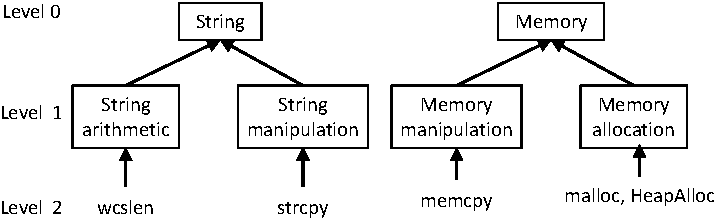
\includegraphics[height=3.5cm, width=8.5cm]{srj-figures/srj-abs-1.pdf} \vspace{-1mm} 
\caption{System API Abstraction Levels}
\label{fig:abs} \vspace{-1mm}
\end{center}
\end{figure}

Note that the function normalization process above is x86 architecture specific, however, a similar approach with some modifications can be successfully applied  to normalize ARM instructions. For example, ARM has different addressing modes compared to x86, which need to be properly handled in normalization process.

\idiomDep{
\begin{MyAlgo}[t]{-4.9cm} %increase or decrease margin, span across columns
\small
 \DontPrintSemicolon
 \KwData{partial trace $\wp$}
 \KwResult{set of data-flow paths $G$}
% \SetKwFunction{algo}{ExtractTracelets}\SetKwFunction{proc}{Extract}
% \SetKwProg{myalg}{Algorithm}{}{}
% \myalg{\algo{$CFG$}}{
  $G \longleftarrow \emptyset$ \;%\tcp*{set of abstract semantic graphs}
 \ForEach{{\upshape instruction} i {\upshape in} $\wp$}{
  %\tcc{write the algo here}
  %$kT \longleftarrow kT \cup Extract(b, k)$\;
  $D_i \longleftarrow  \mathtt{getDef}(i)$\;
  $g \longleftarrow \emptyset$\;
  $j := i.\mathtt{Next}$\tcp*{$j$ is the next instruction after $i$ in $\wp$}
   \ForEach{{\upshape instruction} j {\upshape in} $\wp$}{
   $U_j \longleftarrow  \mathtt{getUse}(j)$\;
   $D_j \longleftarrow  \mathtt{getDef}(j)$\;
   \If{$U_j \in D_i $}{
	   	$g := g \cup {v_i \rightarrow v_j}$\;
   		 \If{$\mathtt{getType}(j) == \mathtt{COPY}$}{
   			$D_i := D_i \cup D_j$\;
   		}
     }
      \If{$D_j \in D_i $}{
	   	$D_i := D_i \setminus D_j$\;
   		}
   		\If{$D_i ==  \emptyset $}{
   			%\If{$g$ {\upshape not in}  $G$}{
   			\If{$\mathtt{isPresent}(g,G) = 0$}{
   		 		$G := G \cup g$\;
   		 	}
	   	   $break$\;
   		}
   }
  }
  \Return ${G}$
  \\
 \caption{Data-flow analysis among instructions using def-use chain \note{seems there is a logic mistake, need to fix }}\label{algo:def-use}
\end{MyAlgo}
}

\idiomDep{
\subsubsection{Idioms Dependency Calculation} \label{subsubsec:dep_cal}
Algorithm \ref{algo:def-use} presents the steps involved in identifying the data dependence between assembly instructions. Here, we define several functions to accomplish our tasks. They are; (1) $\mathtt{getDef(i)}$ returns the variables defined in instruction $i$ (e.g., in `$\mathtt{mov\;eax,ebx}$', the register $\mathtt{eax}$ is defined), (2) $\mathtt{getUse(i)}$ returns the variables used in instruction $i$ (e.g., in the previous instruction, the register $\mathtt{ebx}$ is used), (3) $\mathtt{isPresent(g,G)}$ checks whether the data-flow path $g$ is already present in $G$, where $G$ is a set of extracted data-flow paths, and (4) $\mathtt{getType(i)}$  returns the type of the instruction $i$. At high-level, for each instruction present in the partial trace, we get the variables defined in that instruction, then we iterate through the rest of the instructions to check whether the defined variables are used elsewhere, if found, data dependency between the two instructions is established. Each iteration terminates when (1) it reaches end of the partial trace, or (2) variable defined by instruction $i$ is redefined by another instruction $j$, where $location(i) < location(j)$. Finally, from each data-flow path in $G$, we check for the idioms that are extracted using Algorithm~\ref{algo:idiom-ext}.
}
